\subsection{Grid-Based Surveillance and LoRa Coordination}
\label{subsec:grid_surveillance}

\subsubsection{Search Zone Discretisation}

The surveillance area is defined as a polygon loaded from a mission JSON file. To enable systematic coverage tracking, the zone is discretised into a uniform grid of square cells, each measuring $n \times n$\,m. Then control algorithms operate at the cell level, treating each cell as a discrete unit of space to be visited and monitored.


\begin{figure}[htbp]
    \centering
    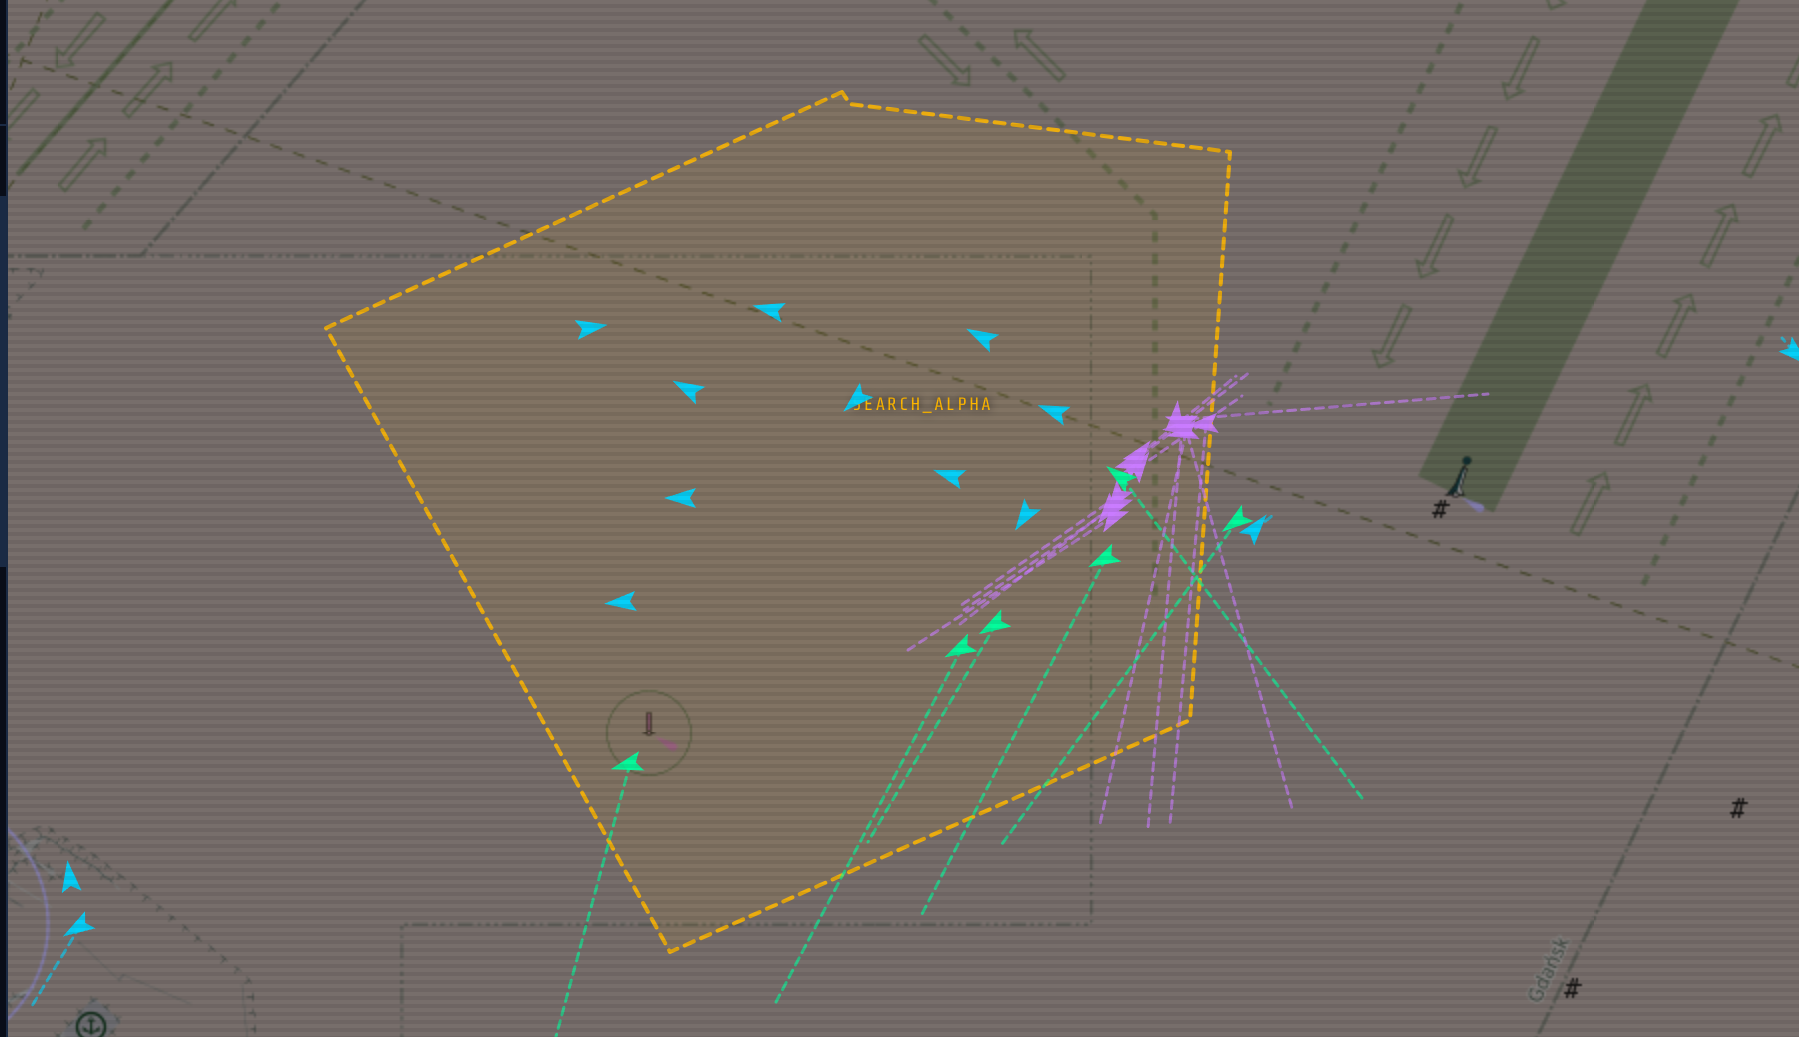
\includegraphics[width=0.6\textwidth]{images/search_zone.png}
    \caption{In this test case, $n = 300$\,m. The cell size represents a balance between the number of cells a swarm of twelve test UAVs must manage: at this resolution the SEARCH\_ALPHA zone in the Gulf of Gda\'nsk yields 698 cells.}
    \label{fig:surveillance_zone}
\end{figure}




Grid construction proceeds as follows. The axis-aligned bounding box of the polygon is computed, and candidate cell centres are placed at half-step offsets from the minimum corner:

\begin{equation}
    \text{lat}_i = \text{lat}_{\min} + \left(i + \tfrac{1}{2}\right) \cdot \frac{d_{\text{cell}}}{m_{\text{lat}}}, \quad
    \text{lon}_j = \text{lon}_{\min} + \left(j + \tfrac{1}{2}\right) \cdot \frac{d_{\text{cell}}}{m_{\text{lon}}}
    \label{eq:cell_centres}
\end{equation}

\noindent where $d_{\text{cell}} = 300$\,m, $m_{\text{lat}} = 111\,320$\,m\,deg$^{-1}$, and $m_{\text{lon}} = 63\,990$\,m\,deg$^{-1}$ (the latter evaluated at latitude $54°$\,N for the Baltic Sea). Each candidate centre is tested for containment within the zone boundary using the standard ray-casting algorithm. Only interior cells are retained; bounding-box cells outside the polygon are discarded.

\subsubsection{Algorithm goal}

Each cell $c$ maintains a single state variable: the Unix timestamp $t_c^{\text{visit}}$ of its most recent visit, initialised to zero (never visited). A drone is considered to have visited cell $c$ when its Kalman-estimated position comes within the arrival threshold $r_{\text{arrive}} = 80$\,m of the cell centre. This method should evenly cover the entire zone, with the swarm collectively minimising the maximum staleness $\tau_{\max} = \max_{c}\, (t_{\text{now}} - t_c^{\text{visit}})$ across all cells. 

\subsubsection{Decentralised Cell Assignment}

Cell assignment is fully decentralised: each drone independently selects its next target without communicating with a central controller. The selection criterion is a scalar score computed for every candidate cell:

\begin{equation}
    s(c) = \tau(c) - P_{\text{contention}} \cdot \mathbf{1}[\text{targeted by neighbour}] - \frac{d(c)}{d_{\max}} \cdot P_{\text{dist}}
    \label{eq:cell_score}
\end{equation}

where $\tau(c)$ is the \emph{staleness} of cell $c$ in seconds (time elapsed since last visit, or $10^6$ if never visited), $P_{\text{contention}} = 120$\,s is a penalty applied when a LoRa neighbour has already claimed the cell as its target, $d(c)$ is the Euclidean distance from the drone's current position to the cell centre, $d_{\max} = 5\,000$\,m is a normalisation constant, and $P_{\text{dist}} = 60$\,s is the maximum distance penalty. The drone selects the cell with the highest score.

This scoring function embodies three competing objectives. The staleness term ensures that cells which have not been visited recently are systematically prioritised, driving the swarm toward complete and uniform temporal coverage. The contention penalty provides implicit coordination: if a neighbour has broadcast its intention to visit a given cell, other drones treat that cell as less attractive, naturally spreading the swarm across the zone without explicit negotiation. The distance penalty serves as a tie-breaker that biases each drone toward nearby cells, reducing unnecessary transit time.

Never-visited cells receive a staleness of $10^6$\,s, which dominates all other terms in Equation~\eqref{eq:cell_score}. This guarantees that initial coverage---visiting every cell at least once---is completed before the swarm begins revisiting cells for temporal surveillance.

\subsubsection{LoRa Beacon Protocol}

Inter-drone coordination relies on LoRa radio communication, which imposes strict payload constraints. Each beacon is encoded as a compact binary structure of at most 36\,bytes, transmitted as a Base64 string (48\,characters). The wire format is defined in Table~\ref{tab:lora_beacon}.

\begin{table}[h]
\centering
\caption{LoRa surveillance beacon wire format (36\,bytes maximum).}
\label{tab:lora_beacon}
\begin{tabular}{llll}
\hline
\textbf{Bytes} & \textbf{Type} & \textbf{Field} & \textbf{Description} \\
\hline
0       & \texttt{uint8}  & \texttt{droneId}      & Sender identifier (0--255) \\
1--2    & \texttt{int16}  & \texttt{targetCell}   & target Cell ID  \\
3--4    & \texttt{int16}  & \texttt{occupiedCell} & current Cell ID \\
5       & \texttt{uint8}  & \texttt{numUpdates}   & visit records (0--6) \\
6--10   & \texttt{uint16} + \texttt{uint24} & \texttt{update[0]} & Cell ID + age in seconds \\
$\vdots$ & $\vdots$ & $\vdots$ & $\vdots$ \\
31--35  & \texttt{uint16} + \texttt{uint24} & \texttt{update[5]} & Cell ID + age in seconds \\
\hline
\end{tabular}
\end{table}

Each beacon includes up to six visit records, each encoding a cell identifier and the time elapsed since that cell was last visited (stored as a 24-bit unsigned integer in seconds, supporting ages up to approximately 194 days). Visit records are ordered by recency: the most recently visited cells are transmitted first. This prioritisation ensures that neighbours learn the freshest information first, which is most actionable for cell-selection decisions.

Beacons are transmitted every 15 control ticks. At a control loop rate of 50\,Hz this corresponds to a broadcast interval of 300\,ms per drone. For a twelve-drone swarm, the aggregate beacon rate is 40 transmissions per second across the network, well within the duty-cycle limitations of LoRa at the spreading factors typical of maritime deployments. For bigger drone swarms, the broadcast interval can be decreased to reduce network congestion, at the cost of slower state propagation.

\subsubsection{Distributed State Fusion}

Upon receiving a state broadcast from a neighbour, each drone performs two operations on its local grid state. First, it records the neighbour's target cell, enabling the contention penalty in Equation~\eqref{eq:cell_score} to discourage duplicate assignments. Second, it merges each reported visit timestamp, accepting the update only if the reported timestamp is more recent than the locally stored value:

\begin{equation}
    t_c^{\text{visit}} \leftarrow \max\!\left(t_c^{\text{visit}},\; t_c^{\text{neighbour}}\right)
    \label{eq:merge}
\end{equation}


The system is robust to drone loss: if a drone fails or leaves communication range, its claimed target cell is simply never visited, causing its staleness to grow until another drone selects it as its highest-scoring target. No explicit failure detection or task reassignment is required.

\subsubsection{Coverage Metric}

System-level performance is quantified by two metrics reported in the drone status output. The \emph{coverage fraction} $\rho$ is the proportion of cells visited at least once:

\begin{equation}
    \rho = \frac{|\{c : t_c^{\text{visit}} > 0\}|}{|C|}
    \label{eq:coverage}
\end{equation}

\noindent where $C$ is the set of all grid cells. The \emph{maximum staleness} $\tau_{\max} = \max_{c \in C}\, \tau(c)$ quantifies the worst-case time since any cell was last visited, which is the primary operational metric for a surveillance mission: it bounds the maximum time interval during which a target could have entered, traversed, and exited any cell undetected.



\begin{figure}[h]

    \subsection{Algorithm Demonstration}
    \centering
 
    % ── Row 1 ─────────────────────────────────────────────────────
    \begin{subfigure}[t]{0.48\textwidth}
        \centering
        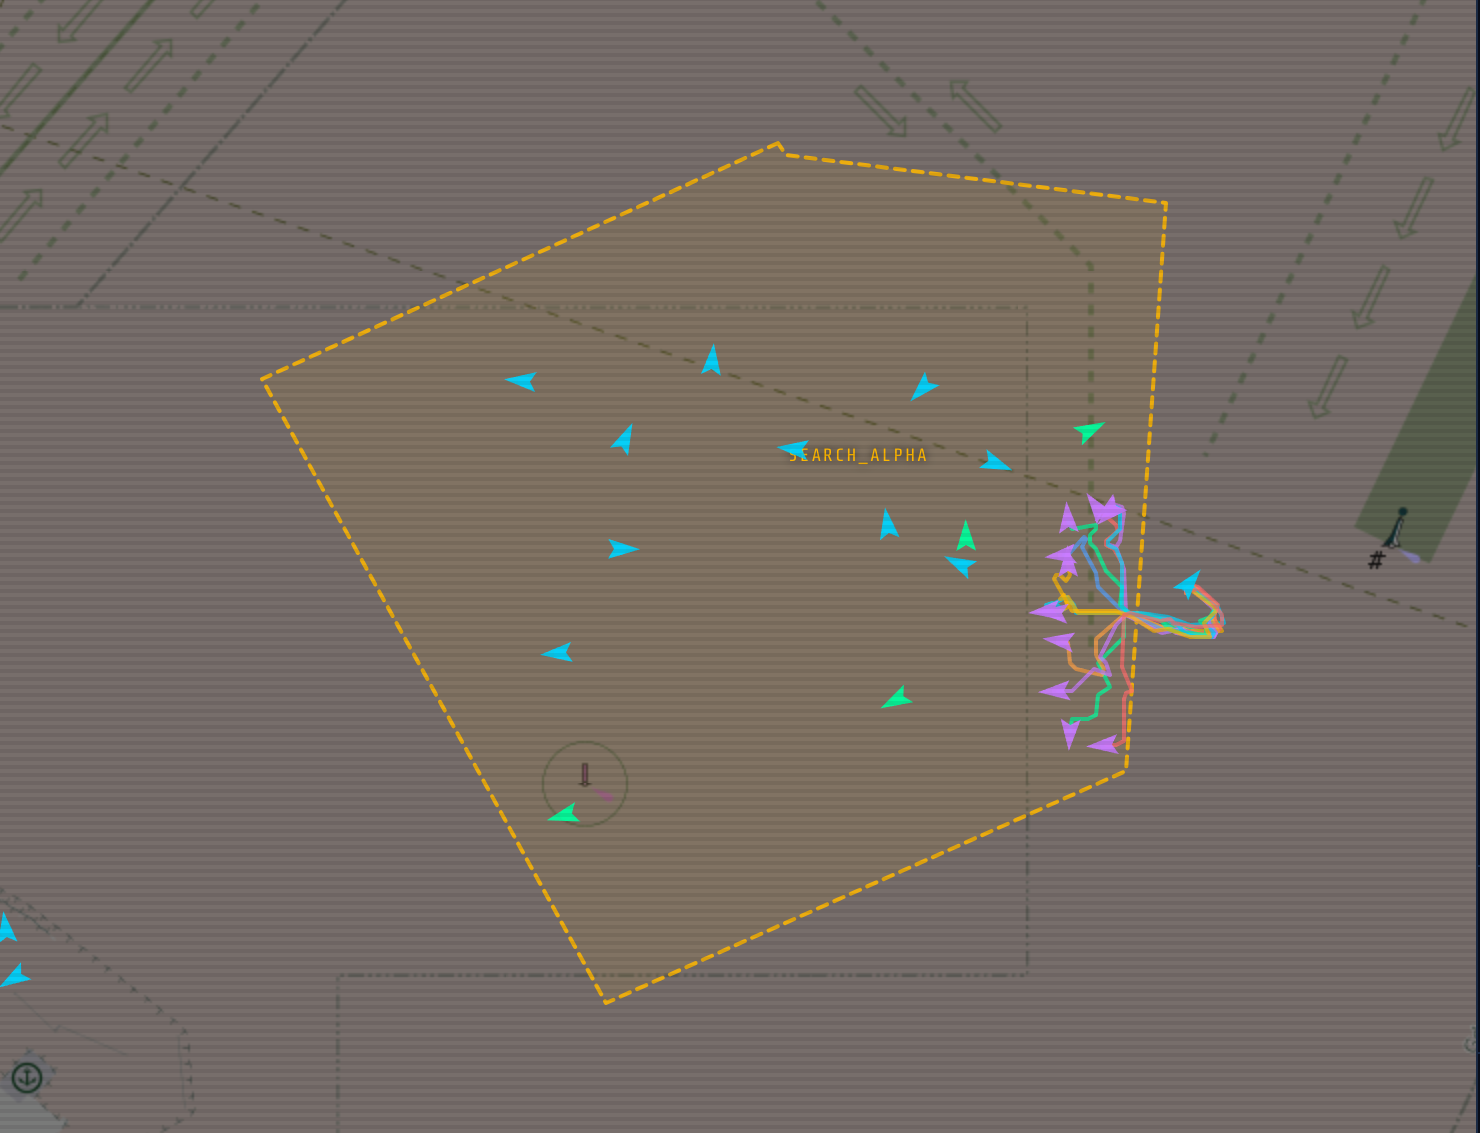
\includegraphics[width=\textwidth]{images/swarm_grid_01.png}
        \caption{Drones entered the zone from the right, then spread out to cover the area.}
        \label{fig:swarm_grid_01}
    \end{subfigure}
    \hfill
    \begin{subfigure}[t]{0.48\textwidth}
        \centering
        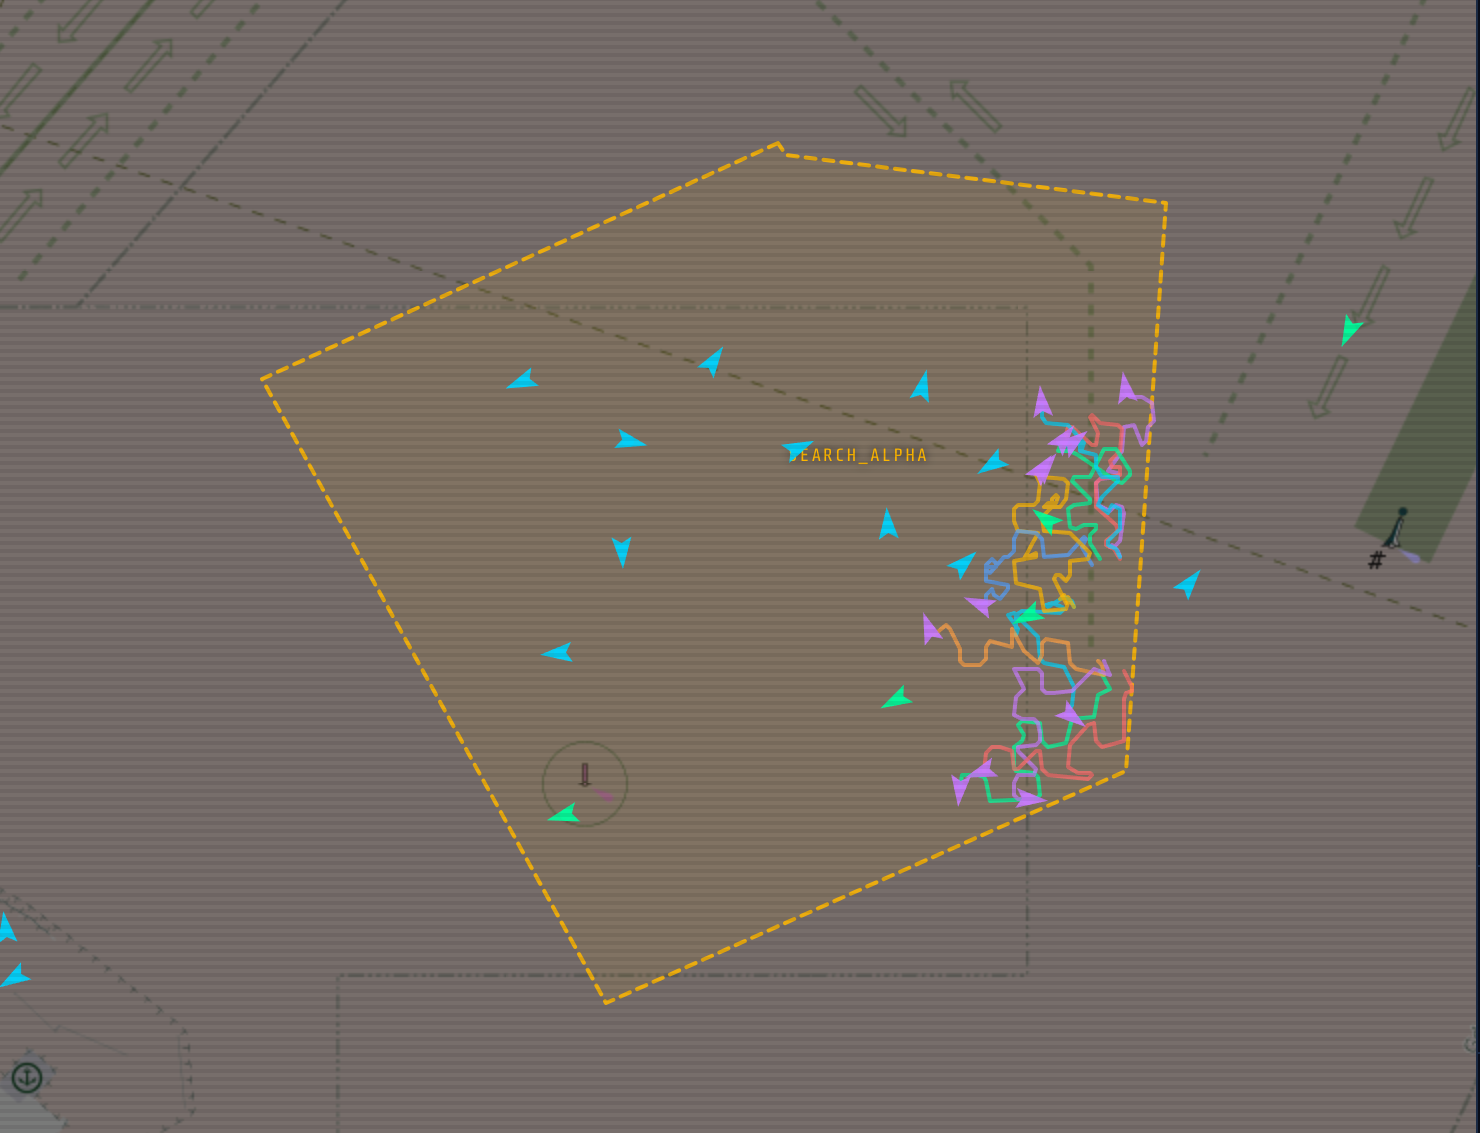
\includegraphics[width=\textwidth]{images/swarm_grid_03.png}
        \caption{Drones are trying to cover the zone as evenly as possible, while avoiding cells targeted by neighbours.}
        \label{fig:swarm_grid_03}
    \end{subfigure}
 
    \vspace{0.5em}
 
    % ── Row 2 ─────────────────────────────────────────────────────
    \begin{subfigure}[t]{0.48\textwidth}
        \centering
        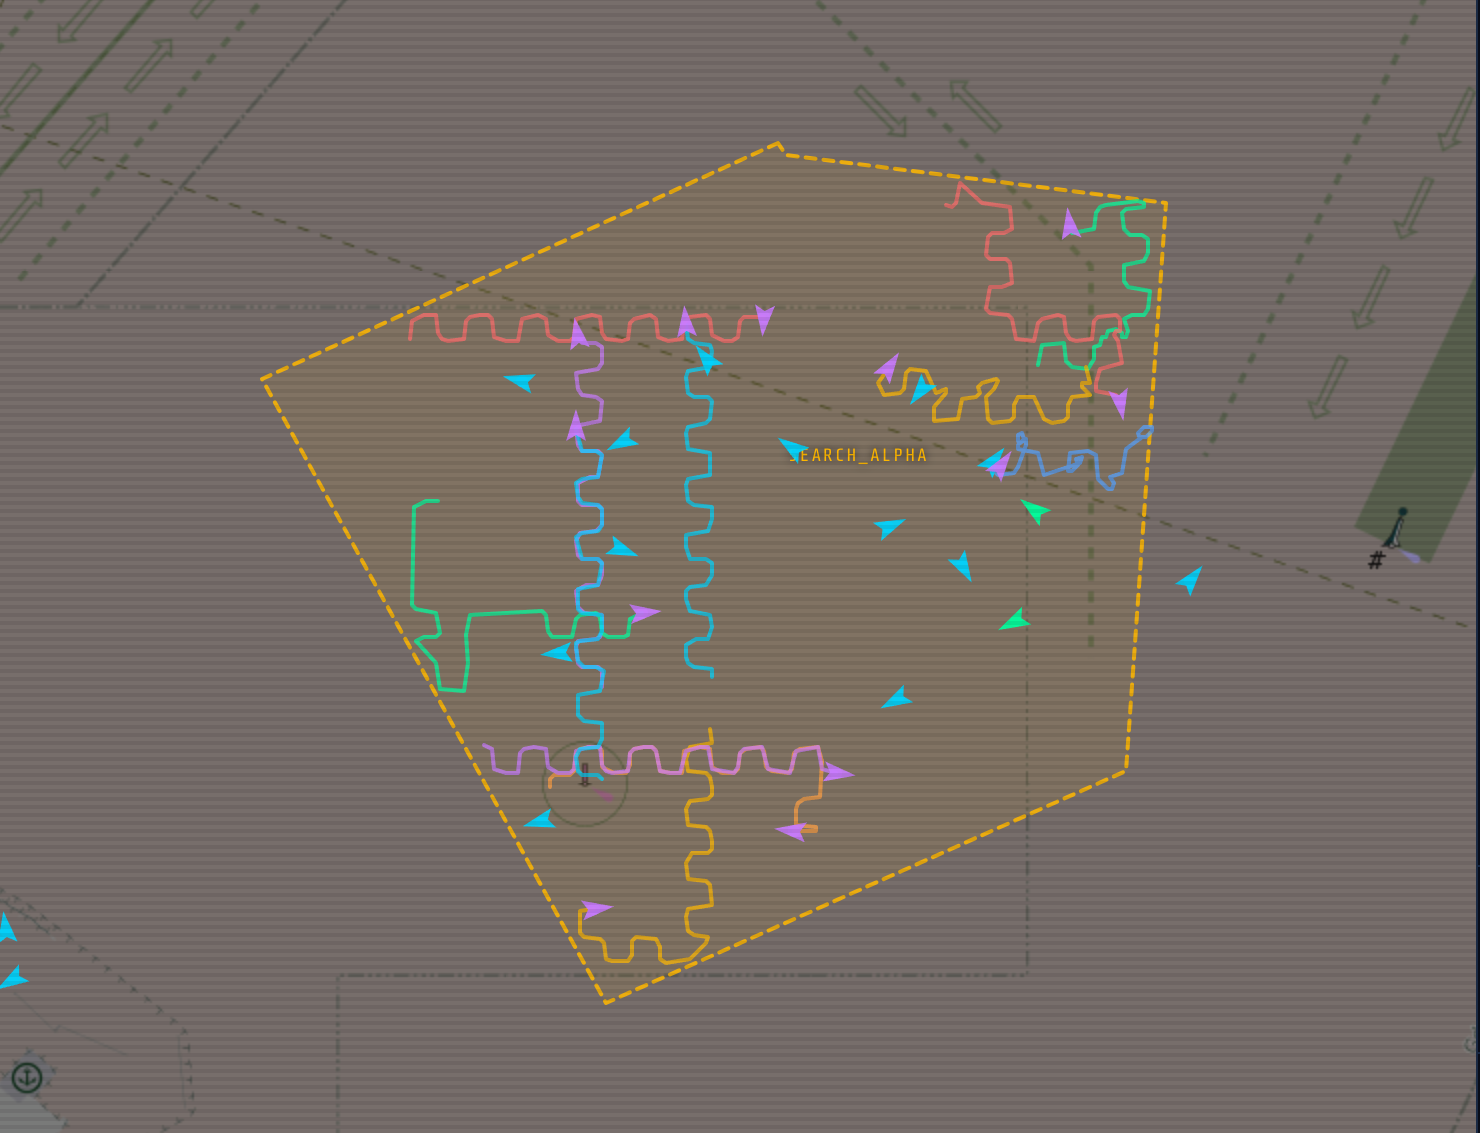
\includegraphics[width=\textwidth]{images/swarm_grid_04.png}
        \caption{Drones are evenly distributed across the zone, with some cells visited more recently than others.}
        \label{fig:swarm_grid_04}
    \end{subfigure}
    \hfill
    \begin{subfigure}[t]{0.48\textwidth}
        \centering
        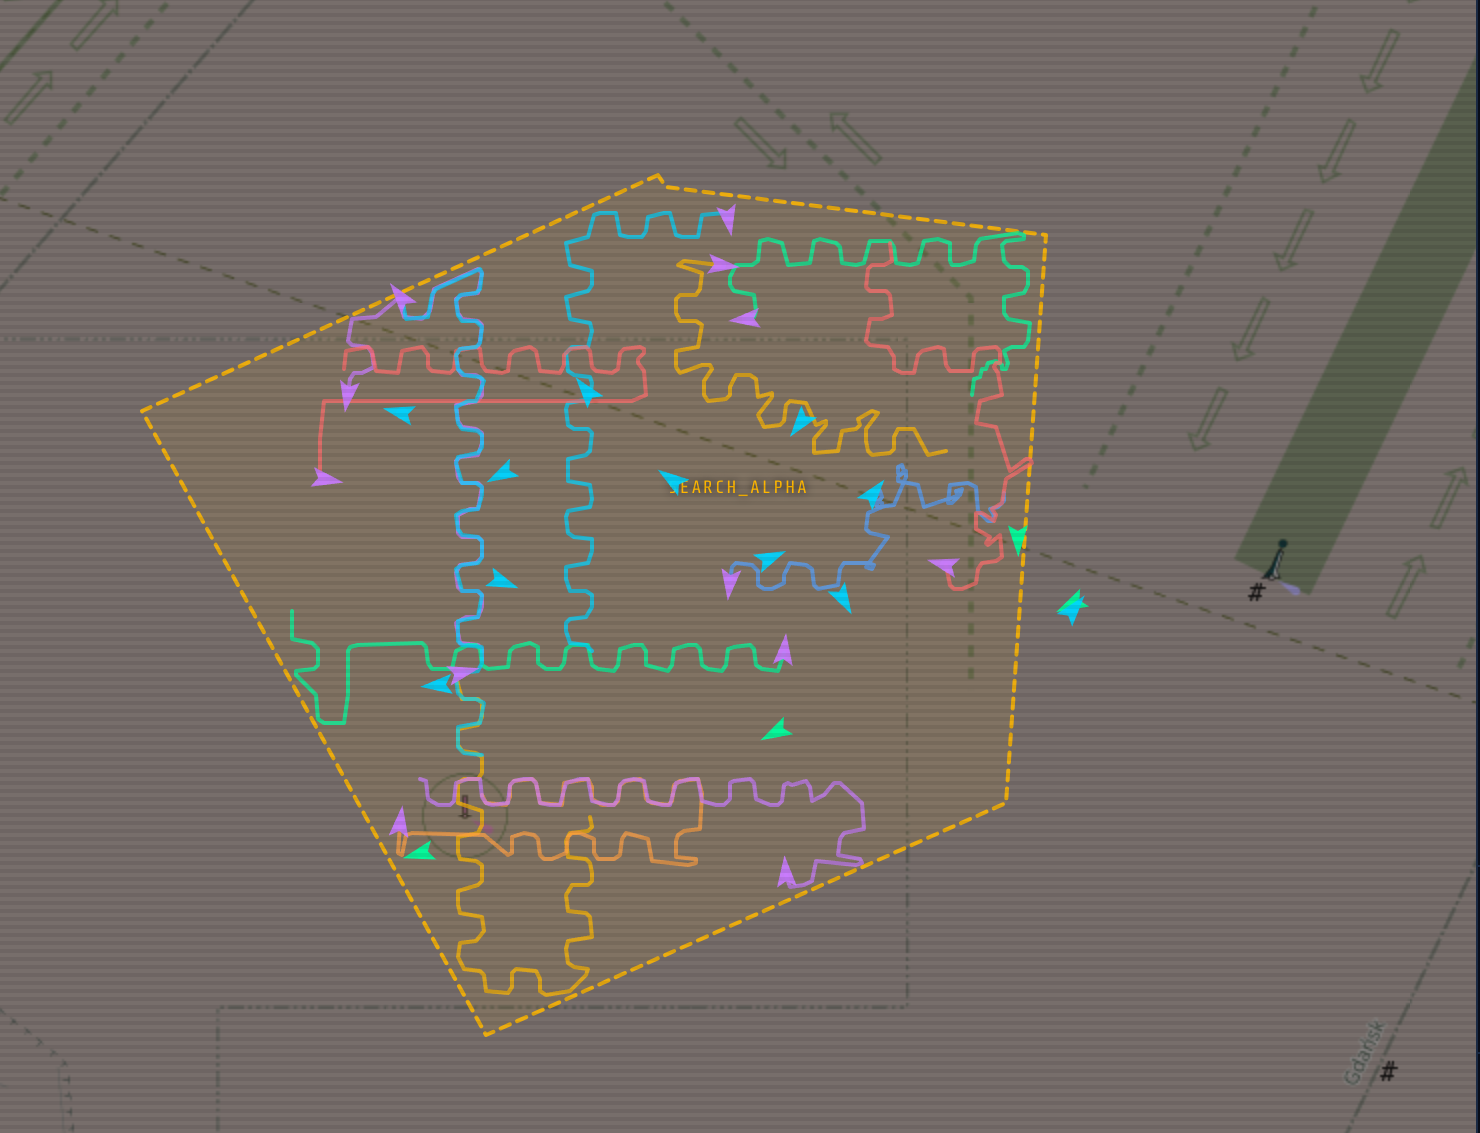
\includegraphics[width=\textwidth]{images/swarm_grid_06.png}
        \caption{Drones now are revisiting cells to maintain coverage.}
        \label{fig:swarm_grid_06}
    \end{subfigure}
 
    \caption{Overall swarm behaviour, drones are trying to cover while avoiding each other and other vessels in the area. For the test I have chosen a anchorage area in the Gulf of Gda\'nsk, which is a busy shipping lane with a high density of vessels.}
    \label{fig:main}
\end{figure}